Edge computing \cite{Edge} is an open platform that integrates network, computing, storage, and application core
capabilities on the edge of the network that is physically close to the data source \cite{Edge2}. It provides
a computing model for edge intelligence services. The location where the edge calculation occurs is
called the edge node, which can be any node between the data generation source and the cloud center
that has computing resources and network resources. The amount of devices connected to the
internet, and as a consequence the amount of data shared, is constantly \cite{DataGrowth} growing and this introduced
a number of different problems that have to be addressed.
\\
\begin{enumerate}
        \item First of all the high amount of traffic flowing in the network is making bandwidth a
              bottleneck for the traditional cloud computing approach.

        \item With the popularity of smart home, video data for many families in the house installation
              network camera, privacy and data security will be a problem since data will be collected
              and directly uploaded to the cloud computing increasing the risk of disclosure of users
              personal data.

        \item As more and more user applications run on cloud servers, the demand for energy consumption
              in large-scale data centers will be difficult to meet in the future. The existing research on
              energy consumption in cloud computing centers focuses on how to improve energy efficiency \cite{EnEff}.
              However,improving energy efficiency alone will not solve the enormous energy consumption
              problem of the data center, which will be more prominent in the environment of all things.
\end{enumerate}

In response to this, the development of the application requirements of the Internet of Everything has
spawned an edge computing model. The edge computing model is a new type of computing model that performs
calculations at the edge of the network. In the edge computing model, the edge device has the processing
capability of performing calculation and data analysis, and migrates some or all of the computing tasks
performed by the original cloud computing model to the network edge device, reducing the computing load
of the cloud server, slowing down the pressure of the network bandwidth, and improving the processing
efficiency of data in the era of Internet of Everything. Edge computing is not to replace the cloud,
but to complement the cloud, providing a better computing platform for related technologies such as mobile
computing and the Internet of Things.

Existing research generally divides the architecture of edge computing from the central network to the
edge of the network into three layers: the cloud computing layer, the edge computing layer, and the ending
layer, as shown in Figure \ref{fig:edge_infr} \cite{IoT,Edge4,Edge5}. Different layers are generally divided according to their computing
and storage capabilities. The computing and storage capabilities of the ending layer, the edge computing
layer, and the cloud computing layer are sequentially increased. In order to achieve intra-layer and
cross-layer communication, each communication technology can be connected by various communication
technologies, including wired communication (such as Ethernet, optical fiber), wireless communication
(such as Bluetooth, LTE, ZigBee, NFC, IEEE802.11a/b), /c/g/c, satellite link or a combination of two
technologies \cite{Communication}. Edge computing extends cloud services to the edge of the network by introducing an edge
layer between the terminal device and the cloud.

\begin{figure}
        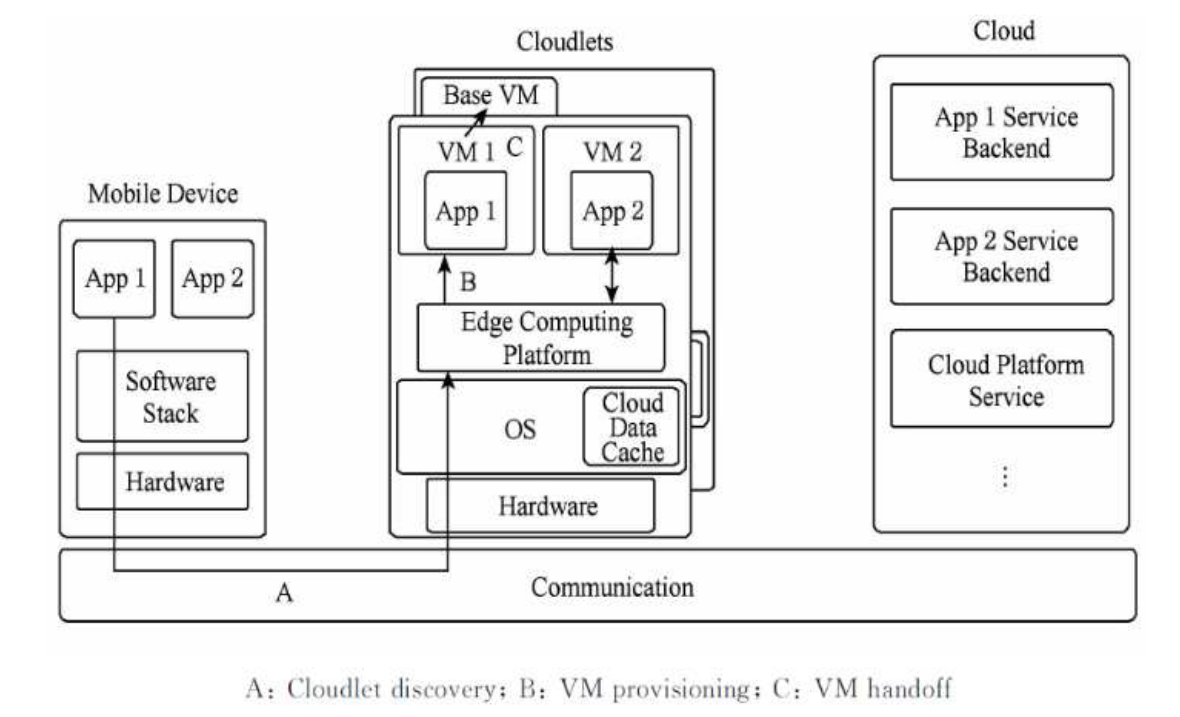
\includegraphics[width=\textwidth]{Images/Edge_infrastructure.png}
        \caption{Edge computing infrastructure.}
        \label{fig:edge_infr}
\end{figure}

% come fitta PAPS in questo
Since some applications can not deal with the high latency from devices to cloud data centers, this approach
can be useful to respect SLA requirements. \\
At the same time, \textit{serverless computing}, also known as Function-as-a-Service (FaaS), offers a new execution model, which enables users
to run their code (a small application dedicated to a specific task; e.g. a single-unit function) without being concerned
about operational issues. This way, the user is relieved from any involvement in the server provisioning and resource
management. Serverless applications are intended to be event-driven and stateless.
For example, FaaS could be instantiated (triggered by the described condition) to execute a predefined function
and shut down when finished. In a commercial system, a user is charged on a per-invocation basis, without paying
for unused or idle resources. Being supported by unlimited Cloud resources, serverless computing represents a form
of utility computing with access to elastic scaling via available on-demand computational resources.\cite{Serverless} \\
Serverless computing is becoming more and more popular, since it allows the developer to focus on the development of an application
while ignoring the infrastructure on which the function will be deployed. With this paradigm, the main
system can dynamically allocate machine resources according to the specific needs of the final application and
being sure that the application SLA will be respected.

To easily manage cloud applications, virtualization results to be the best technology mainly in the form of
\textit{containerization.} Often, the management of cluster of containers becomes essential and the orchestration of the
construction and deployment becomes a central problem.\\
A container holds packaged self-contained, ready-to-deploy parts of applications and, if necessary, middleware and business
logic (in binaries and libraries) to run the applications. Tools like Docker are built around container engines where
containers act as portable means to package applications. This results in the need to manage dependencies between containers
in multi-tier applications. An orchestration plan can describe components, their dependencies and their lifecycle in a layered plan.
To interconnect multiple containers, an \textit{orchestrator} is used. We define orchestration as constructing
and continuously managing possibly distributed clusters of container-based software applications. Container orchestration
allows users to define how to coordinate the containers in the cloud when a multi-container application is deployed.
Container orchestration defines not only the initial deployment of containers, but also the management of the multi-containers
as a single entity. It takes care of availability, scaling and networking of containers. Essentially cloud-based container
construction is a form of orchestration within the distributed cloud environment.\cite{Containers}

In this context, PAPS (Partitioning, Allocation, Placement and Scaling), a framework that tries to
tackle the challenges related to the management of edge computing infrastructures,
is trying to automate the allocation of serverless function and the management of large scale edge topologies.
It should be able to give an optimal allocation for a given workload, but also
to react to unpredictable workload fluctuations that characterize this type of networks.
An initial prototype of the framework was already produced, as presented in PAPS \cite{PAPS} paper,
it uses PeerSim \footnote{ http://peersim.sourceforge.net/} to simulate a network behavior and in which
the serverless functions are implemented as Java threads. The actual workload of the system is then simulated
using a probability distribution.
% nostra implementazione
In this paper we will present our work on PAPS, it mainly consists on a research phase in which we
analyzed the documentation of some support frameworks, such as OpenFaas, OpenWhisk and Kubernetes, with the
aim to simplify the deployed of a real world implementation. Based on the initial prototype we identified a
general idea of how all PAPS phases will need to be implemented and integrated with the external frameworks and
in the end we also developed an implementation of the partition phase.

% struttura PAPS
The rest of the paper is organized as follows. Section \ref{sect:paps} presents the theoretical structure of the
framework which was the starting point of our work. Section \ref{sect:research} describes how frameworks and tools
used in the actual implementation have been chosen among all the possible choices. Sections \ref{sect:generalImpl}
and \ref{sect:implementation} go more in detail about the general implementation idea for the overall framework and
more in details how a prototype for the partition phase has been created. Section \ref{sect:testing} describes the tests
made on our implementation. Section \ref{sect:conclusion} concludes the paper.
